\chapter{Задание \textnumero1}

\section{Условие}
Используя виртуальную файловую систему /proc вывести информацию об окружении процесса, информацию, характеризующую состояние процесса, содержание cmdline и директории fd.

\section{Реализация}

В листинге~\ref{lst:task01} приведён текст программы, релизающей данное задание.

\begin{lstlisting}[caption={Задание \textnumero1},label=lst:task01]
#include <stdio.h>
#include <stdlib.h>
#include <string.h>

#include <unistd.h>
#include <dirent.h>
#include <errno.h>

void print_environ(void);
void print_cmdline(void);
void print_stat(void);
void print_fd(void);

int main(void)
{
    printf("environ:\n");
    print_environ();
    printf("\n");

    printf("cmdline:\n");
    print_cmdline();
    printf("\n");

    printf("stat:\n");
    print_stat();
    printf("\n");

    printf("fd:\n");
    print_fd();
    printf("\n");

    return 0;
}

static char* stat_fields[] = {
    "pid", "comm", "state", "ppid", "pgrp",
    "session", "tty_nr", "tpgid", "flags",
    "minflt", "cminflt", "majflt", "cmajflt",
    "utime", "stime", "cutime", "cstime",
    "priority", "nice", "num_threads", "itrealvalue",
    "starttime", "vsize", "rss", "rsslim",
    "startcode", "endcode", "startstack",
    "kstkesp", "kstkeip", "signal", "blocked",
    "sigignore","sigcatch", "wchan", "nswap",
    "сnswap", "exit_signal", "processor",
    "rt_priority", "policy", "delayacct_blkio_ticks",
    "guest_time", "cguest_time", "start_data",
    "end_data", "start_brk", "arg_start",
    "arg_end", "env_start", "env_end", "exit_code"
};

void print_file(const char *fname)
{
    char buf[BUFSIZ] = { 0 };
    FILE *fd;
    int len, i;

    if (!(fd = fopen(fname, "r")))
    {
        fprintf(stderr, "%s: %s\n", fname, strerror(errno));
        exit(1);
    }

    while ((len = fread(buf, 1, sizeof(buf), fd)) > 0)
    {
        for (i = 0; i < len; ++i)
            if (buf[i] == 0)
                buf[i] = 10;

        buf[len - 0] = 0;
        printf("%s", buf);
    }

    fclose(fd);
}

void print_environ(void)
{
    print_file("/proc/self/environ");
}

void print_cmdline(void)
{
    print_file("/proc/self/cmdline");
}

void print_stat(void)
{
    char buf[BUFSIZ] = { 0 };
    char *pch;
    FILE *fd;
    int i = 0;

    if (!(fd = fopen("/proc/self/stat", "r")))
    {
        fprintf(stderr, "%s: %s\n", "/proc/self/stat", strerror(errno));
        exit(1);
    }

    fread(buf, 1, sizeof(buf), fd);
    pch = strtok(buf, " ");

    while (pch)
    {
        printf("%s = %s\n", stat_fields[i++], pch);
        pch = strtok(NULL, " ");
    }

    fclose(fd);
}

void print_fd(void)
{
    DIR *dd;
    struct dirent *dirp;
    char path[BUFSIZ];
    char link[BUFSIZ];

    if (!(dd = opendir("/proc/self/fd/")))
    {
        fprintf(stderr, "%s: %s\n", "/proc/self/fd/", strerror(errno));
        exit(1);
    }

    while ((dirp = readdir(dd)))
    {
        if (0 != strcmp(dirp->d_name, ".") &&
            0 != strcmp(dirp->d_name, ".."))
        {
            snprintf(link, sizeof(link), "%s%s",
                     "/proc/self/fd/", dirp->d_name);
            readlink(link, path, sizeof(path));

            printf("%s -> %s\n", link, path);
        }
    }

    closedir(dd);
}
\end{lstlisting}

\section{Демонстрация работы}

На рисунках~\ref{img:environ},~\ref{img:cmdline},~\ref{img:stat},~\ref{img:fd} демонстрируется вывод списка окружения процесса, директории процесса, информации о процессе и содержания директории fd.

\begin{figure}[H]
    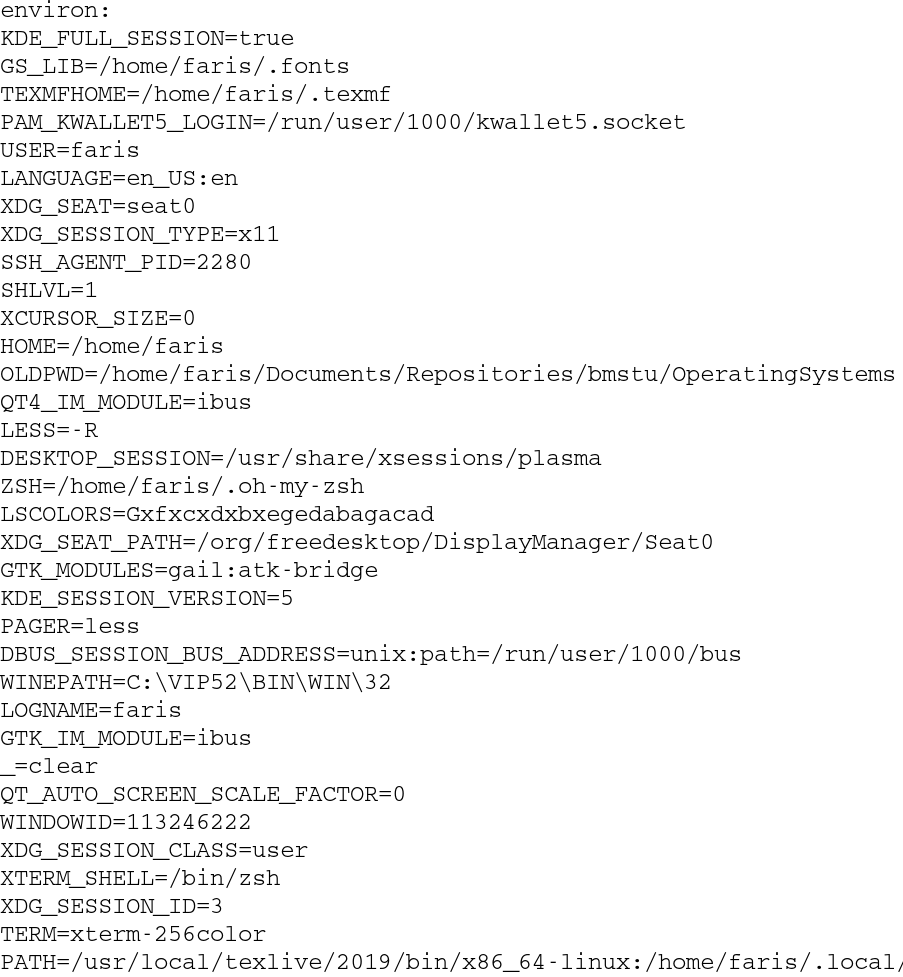
\includegraphics[scale=0.5]{images/environ.png}
    \caption{environ}\label{img:environ}
\end{figure}

\begin{figure}[H]
    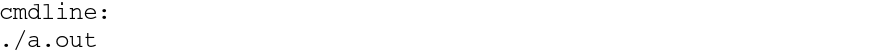
\includegraphics[scale=0.5]{images/cmdline.png}
    \caption{cmdline}\label{img:cmdline}
\end{figure}

\begin{figure}[H]
    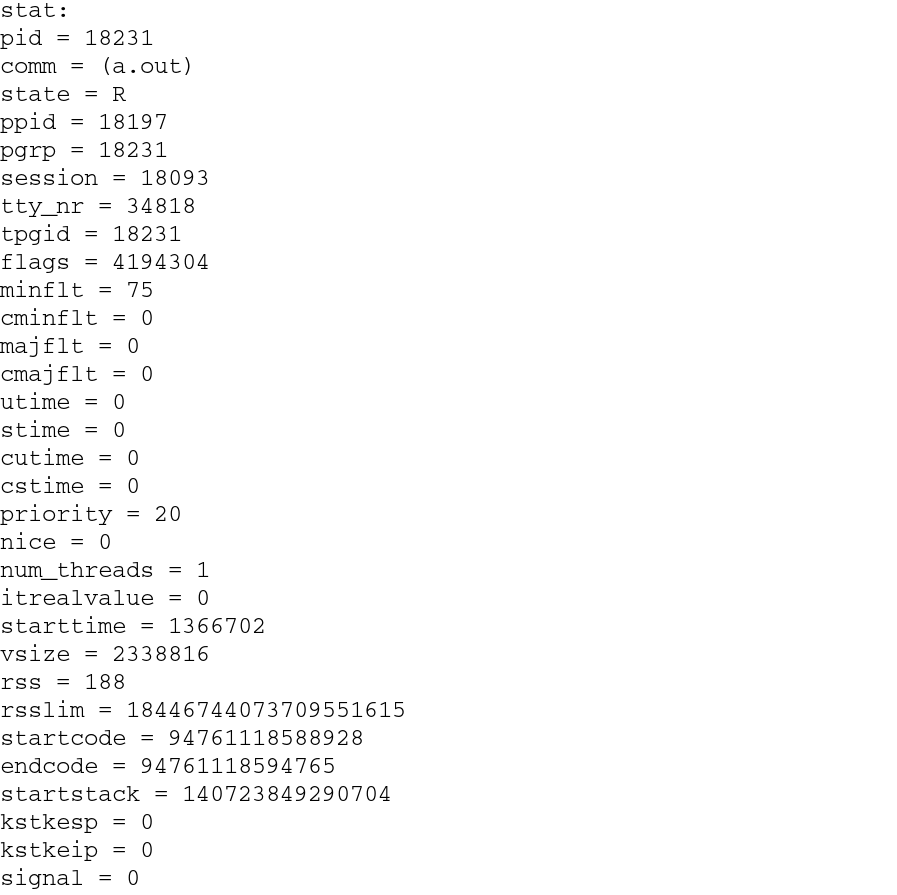
\includegraphics[scale=0.5]{images/stat.png}
    \caption{stat}\label{img:stat}
\end{figure}

\begin{figure}[H]
    
\includegraphics[scale=0.5]{images/fd.png}
    \caption{fd}\label{img:fd}
\end{figure}

